\documentclass[11pt,letterpaper]{article}

\addtolength{\oddsidemargin}{-.875in}
\addtolength{\evensidemargin}{-.875in}
\addtolength{\textwidth}{1.75in}

\addtolength{\topmargin}{-.875in}
\addtolength{\textheight}{1.75in}

\usepackage[utf8]{inputenc}
\usepackage{caption} % for table captions
\usepackage{amsmath} % for multi-line equations and piecewises
\DeclareMathOperator{\sign}{sign}
\usepackage{graphicx}
\usepackage{relsize}
\usepackage{xspace}
\usepackage{verbatim} % for block comments
\usepackage{subcaption} % for subfigures
\usepackage{enumitem} % for a) b) c) lists
\newcommand{\Cyclus}{\textsc{Cyclus}\xspace}%
\newcommand{\Cycamore}{\textsc{Cycamore}\xspace}%
\newcommand{\deploy}{\texttt{d3ploy}\xspace}%
\newcommand{\Deploy}{\texttt{D3ploy}\xspace}%
\usepackage{tabularx}
\usepackage{color}
\usepackage{multirow}
\usepackage{float} 
\usepackage[acronym,toc]{glossaries}
%\newacronym{ANL}{ANL}{Argonne National Laboratory}
\newacronym{B4C}{B4C}{boron carbide}
\newacronym{BC}{BC}{boundary condition}
\newacronym{BOC}{BOC}{beginning of equilibrium cycle}
\newacronym{BSD}{BSD}{Berkeley Software Distribution}
\newacronym{BWR}{BWR}{Boiling Water Reactor}
\newacronym{CAISO}{CAISO}{California ISO}
\newacronym{CEA}{CEA}{Commissariat a l'Energie Atomique}
\newacronym{CFD}{CFD}{computational fluid dynamics}
\newacronym{CO2}{CO$_2$}{carbon dioxide}
\newacronym{CR}{CR}{control rod}
\newacronym{CRP}{CRP}{Coordinated Research Project}
\newacronym{CZP}{CZP}{Cold Zero Power}
\newacronym{DCC}{DCC}{depressurized conduction cool-down}
\newacronym{DOE}{DOE}{Department of Energy}
\newacronym[\glslongpluralkey={degrees of freedom}]{DoF}{DoF}{degree of freedom}
\newacronym{EOC}{EOEC}{end of equilibrium cycle}
\newacronym{FCEV}{FCEV}{Fuel Cell Electric Vehicle}
\newacronym{FDM}{FDM}{Finite Difference Method}
\newacronym{FEM}{FEM}{Finite Element Method}
\newacronym{FVM}{FVM}{Finite Volume Method}
\newacronym{FSV}{FSV}{Fort St. Vrain}
\newacronym[\glslongpluralkey={greenhouse gases}]{GHG}{GHG}{greenhouse gas}
\newacronym{GRS}{GRS}{Gesellschaft für Anlagen und Reaktorsicherheit}
\newacronym{H2}{H$_2$}{hydrogen}
\newacronym{He}{He}{helium}
\newacronym{HFP}{HFP}{Hot Full Power}
\newacronym{HPCC}{HPCC}{high pressure conduction cool-down}
\newacronym{HTE}{HTE}{High-Temperature Electrolysis}
\newacronym{HTGR}{HTGR}{High-Temperature Gas-Cooled Reactor}
\newacronym{HTR}{HTR}{High Temperature Reactor}
\newacronym{HTTR}{HTTR}{High Temperature Test Reactor}
\newacronym{HZDR}{HZDR}{Helmholtz-Zentrum Dresden-Rossendorf}
\newacronym{IAEA}{IAEA}{International Atomic Energy Agency}
\newacronym{icap}{iCAP}{Illinois Climate Action Plan}
\newacronym{INL}{INL}{Idaho National Laboratory}
\newacronym{IPyC}{IPyC}{inner pyrolytic carbon}
\newacronym{JFNK}{JFNK}{Jacobian-Free Newton-Krylov}
\newacronym{KAERI}{KAERI}{Korea Atomic Energy Research Institute}
\newacronym{Keff}{K$_{eff}$}{multiplication factor}
\newacronym{LBP}{LBP}{Lumped Burnable Poison}
\newacronym{LGPL}{LGPL}{Lesser GNU Public License}
\newacronym{LOCA}{LOCA}{loss of coolant accident}
\newacronym{LPCC}{LPCC}{low pressure conduction cool-down}
\newacronym{LTE}{LTE}{Low-Temperature Electrolysis}
\newacronym{LWR}{LWR}{Light Water Reactor}
\newacronym{MC}{MC}{Monte Carlo}
\newacronym{MHTGR}{MHTGR}{Modular High-Temperature Gas-Cooled Reactor}
\newacronym{MOC}{MOC}{middle of equilibrium cycle}
\newacronym{MOOSE}{MOOSE}{Multi-physics Object-Oriented Simulation Environment}
\newacronym{MPI}{MPI}{Message Passing Interface}
\newacronym{MSR}{MSR}{Molten Salt Reactor}
\newacronym{MTD}{MTD}{Champaign-Urbana Mass Transit District}
\newacronym{NEA}{NEA}{Nuclear Energy Agency}
\newacronym{NEM}{NEM}{Nodal Expansion Method}
\newacronym{NGNP}{NGNP}{Next Generation Nuclear Power}
\newacronym{NRC}{NRC}{Nuclear Regulatory Commission}
\newacronym{NSC}{NSC}{Nuclear Science Committee}
\newacronym{OECD}{OECD}{Organisation for Economic Co-operation and Development}
\newacronym{OPyC}{OPyC}{outer pyrolytic carbon}
\newacronym{ORNL}{ORNL}{Oak Ridge National Laboratory}
\newacronym{OS}{OS}{Operator-Splitting}
\newacronym{PBMR}{PBMR}{Pebble Bed Modular Reactor}
\newacronym{PDE}{PDE}{Partial Differential Equation}
\newacronym{PMR}{PMR}{Prismatic Modular Reactor}
\newacronym{PV}{PV}{photovoltaics}
\newacronym{RSC}{RSC}{Reserve Shutdown Control}
\newacronym{RSD}{RSD}{Relative Standard Deviation}
\newacronym{SD}{SD}{Standard Deviation}
\newacronym{SI}{SI}{Sulfur-Iodine}
\newacronym{SiC}{SiC}{silicon carbide}
\newacronym{SMR}{SMR}{Small Modular Reactor}
\newacronym{SNU}{SNU}{Seoul National University}
\newacronym{SOEC}{SOEC}{Solid Oxide Electrolysis Cells}
\newacronym{TIP}{TIP}{transverse integration procedure}
\newacronym{TRISO}{TRISO}{Tristructural Isotropic}
\newacronym{UIUC}{UIUC}{University of Illinois at Urbana-Champaign}
\newacronym{UNIST}{UNIST}{Ulsan National Institute of Science and Technology}
\newacronym{UK}{UK}{United Kingdom}
\newacronym{UMICH}{UMICH}{University of Michigan}
\newacronym{US}{US}{United States}
\newacronym{VHTR}{VHTR}{Very High Temperature Gas Cooled Reactor}
%\newacronym{<++>}{<++>}{<++>}
%\newacronym{<++>}{<++>}{<++>}

\definecolor{bg}{rgb}{0.95,0.95,0.95}
\newcolumntype{b}{X}
\newcolumntype{f}{>{\hsize=.15\hsize}X}
\newcolumntype{s}{>{\hsize=.5\hsize}X}
\newcolumntype{m}{>{\hsize=.75\hsize}X}
\newcolumntype{r}{>{\hsize=1.1\hsize}X}
\usepackage{titling}
\usepackage[hang,flushmargin]{footmisc}
\renewcommand*\footnoterule{}
\usepackage{tikz}

\usetikzlibrary{shapes.geometric,arrows}
\tikzstyle{process} = [rectangle, rounded corners, 
minimum width=1cm, minimum height=1cm,text centered, draw=black, 
fill=blue!30]
\tikzstyle{arrow} = [thick,->,>=stealth]

\graphicspath{}

\begin{document}

\section{MOOSE}

\gls{MOOSE} purpose is to support the development of engineering analysis applications.
It provides a framework where the applications share a common code base, which facilitates relatively easy coupling \cite{novak_pronghorn_2018}.
\gls{MOOSE} utilizes the mathematical structure present in \gls{JFNK} methods.
\gls{JFNK} methods are synergistic combinations of Newton-type methods for superlinearly convergent solution of nonlinear equations and Krylov subspace methods for solving the Newton correction equations.
The link between the two methods is the Jacobian-vector product.
\gls{JFNK} methods compute such product approximately without forming and storing the elements of the true Jacobian \cite{knoll_jacobian-free_2004}.

\gls{MOOSE} modularizes physics expressions into "Kernels".
Kernels are C++ classes that contain methods for computing residual and Jacobian contributions corresponding to individual pieces of governing equations \cite{lindsay_introduction_2018}.
This modularization allows for rapid production of new simulation tools.

% All codes use MPI for parallel communication and allow for deployement on massively-parallel cluster-computing platforms.
% MOOSE applications by default use monolithic and implicit methods ideal for closely-coupled and multi-scale physics.

\section{Moltres}

Moltres \cite{lindsay_introduction_2018} is a \gls{MOOSE} based application originally designed for modeling fluid-fuelled \glspl{MSR}.

This simulation tool is open source and solves arbitrary-group neutron diffusion, precursor, and temperature governing equations.

Its openness is a defining characteristic and promotes quality through transparency and ease of peer review.
It uses git for version control, integration testing to protect developed physics capabilities, and a C++ object-oriented design to enable extension and code reuse.

Being a \gls{MOOSE} based application allows it to run on a single mesh in anywhere from one to three dimensions.
The code uses MPI for parallel communication and allows for deployment on massively-parallel cluster-computing platforms.

Moltres can solve the equations in a fully-coupled way or solve each system independently allowing for great flexibility and making it applicable to a wide range of nuclear engineering problems.

\subsection{Neutronics}

Equations \ref{eq:diffusion} and \ref{eq:precursors} describe the time dependent behavior of the neutronics.

\begin{align}
        \frac{1}{v_g}\frac{\partial}{\partial t} \phi_g &= \nabla \cdot D_g
        \nabla \phi_g - \Sigma_g^r \phi_g \sum_{g \ne g'}^G
        \Sigma_{g'\rightarrow g}^s \phi_{g'} + \notag\\
        &\phantom{{}=1}\chi_g^p \sum_{g' = 1}^G (1 - \beta) \nu \Sigma_{g'}^f \phi_{g'} + 
        \chi_g^d \sum_i^I \lambda_i C_i
\label{eq:diffusion}
        \intertext{where}
        v_g &= \mbox{group $g$ neutron speed} \\
        \phi_g &= \mbox{group $g$ neutron flux} \\
        t &= \mbox{time} \\
        D_g &= \mbox{group $g$ diffusion coefficient} \\
        \Sigma_g^r &= \mbox{group $g$ macroscopic removal cross-section} \\
        \Sigma_{g'\rightarrow g}^s &= \mbox{group $g'$ to group $g$ macroscopic scattering} \notag \\
		&\phantom{{}=1} \mbox{cross-section}\\
        \chi_g^p &= \mbox{group $g$ prompt fission spectrum} \\
        G &= \mbox{number of discrete energy groups} \\
        \nu &= \mbox{number of neutrons produced per fission} \\
        \Sigma_g^f &= \mbox{group $g$ macroscopic fission cross-section} \\
        \chi_g^d &= \mbox{group $g$ delayed fission spectrum} \\
        I &= \mbox{number of delayed neutron precursor groups} \\
        \beta &= \mbox{delayed neutron fraction}\\
        \lambda_i &= \mbox{average decay constant of delayed neutron} \notag\\
        &\phantom{{}=1} \mbox{precursors in precursor group $i$} \\
        C_i &= \mbox{concentration of delayed neutron precursors} \notag \\
        &\phantom{{}=1} \mbox{in precursor group $i$}.
\end{align}

\begin{align}
        \frac{\partial C_i}{\partial t} &= \sum_{g'= 1}^G \beta_i \nu
        \Sigma_{g'}^f \phi_{g'} - \lambda_i C_i
\label{eq:precursors}
\end{align}

For the eigenvalue calculations, the equations lose the time dependent behavior.
Using \ref{eq:chit} we combine both equations. 
We introduce the parameter $k_{eff}$ that divides the fission term obtaining equation \ref{eq:eigenvalue}.

\begin{align}
	\chi_g^t = \chi_g^p (1 - \beta) + \chi_g^d \sum_i^I \beta_i \\
\label{eq:chit}
    \nabla & \cdot D_g \nabla \phi_g - \Sigma_g^r \phi_g + \sum_{g \ne g'}^G
    \Sigma_{g'\rightarrow g}^s \phi_{g'} + \notag\\
    &\phantom{{}=1}\chi_g^t \sum_{g' = 1}^G \frac{1}{k_{eff}}\nu \Sigma_{g'}^f \phi_{g'}
\label{eq:eigenvalue}
\end{align}

% Boundary conditions

Vacuum boundary conditions:

There are no incoming neutrons at a vacuum boundary.
The incoming current density $J^-(r_s, t) = 0$.
In diffusion theory $J^-(r_s, t)$ is defined as

\begin{align}
    J^-(r_s, t) = \frac{1}{4} \phi(r_s, t) + \frac{D}{2} \hat{n_s} \cdot \nabla \phi (r_s, t) = 0
\label{eq:vacuumbc1}
\end{align}


% This might change: if I add the validation in the thesis
The cross sections are input data that has to be previously generated.
In this work, we use \textbf{Serpent} to generate the cross sections.

\subsection{Thermal-Hydraulics}

The governing equation for the temperature in the fuel is

% This might be missing the nt_scale coefficient
\begin{align}
	\rho_f & c_{p,f} \frac{\partial}{\partial t} T_f = \nabla k_f \nabla T_f + Q_f
\label{eq:tempfuel}
	Q_f &= \sum_{g = 1}^{G} \epsilon_g^f \Sigma_g^f \phi_g
\label{eq:heatsource}

    \intertext{where}
    rho_f &= \mbox{fuel density} \\
    c_{p,f} &= \mbox{fuel specific heat capacity} \\
    k_f &= \mbox{fuel thermal conductivity } \\
    T_f &= \mbox{fuel temperature} \\
    Q_f &= \mbox{volumetric heat source} \\
    \epsilon_g^f &= \mbox{energy released per fission} \\
    \Sigma_g^f &= \mbox{group $g$ macroscopic fission cross-section} \\
    \phi_g &= \mbox{group $g$ neutron flux.} \\  
\end{align}

The governing equation for the temperature in the moderator and reflectors is

\begin{align}
	\rho_i & c_{p,i} \frac{\partial}{\partial t} T_i = \nabla k_i \nabla T_i
\label{eq:tempgraphite}
    \intertext{where}
    i &= \mbox{m: moderator, r: reflector} \\
    rho_i &= \mbox{material $i$ density} \\
    c_{p,i} &= \mbox{material $i$ specific heat capacity} \\
    k_i &= \mbox{material $i$ thermal conductivity} \\
    T_i &= \mbox{material $i$ temperature.} \\
\end{align}

The governing equations of the coolant are

\begin{align}
	\frac{\partial} \rho + \nabla \cdot (\rho u) = 0 \\
	\label{eq:continuity}
	
	\rho_c & c_{p,c} \left( \frac{\partial}{\partial t} T_c + u \nabla T_c \right) = \nabla k_c \nabla T_c
	\label{eq:temperature}

    \intertext{where}
    rho_c &= \mbox{coolant density} \\
    u &= \mbox{coolant velocity} \\
    c_{p,c} &= \mbox{coolant specific heat capacity} \\
    k_c &= \mbox{coolant thermal conductivity} \\
    T_c &= \mbox{coolant temperature.} \\

\end{align}

In the steady-state limit, equation \ref{eq:continuity} becomes

\begin{align}
	\rho u & = G = \mbox{constant}. \\
	\label{eq:continuity2}
\end{align}

Introducing equation \ref{eq:continuity2} into \ref{eq:temperature} gives

\begin{align}
	\rho_c & c_{p,c} \frac{\partial}{\partial t} T_c + c_{p,c} G \nabla T_c = \nabla k_c \nabla T_c
	\label{eq:temperature2}
\end{align}

% How to obtain the constants and the values ?

\section{Serpent}

The Serpent Monte Carlo Code is a three-dimensional continuous-energy neutron transport code developed at the VTT Technical Research Centre of Finland.
It is capable of simulating various fuel assembly geometries and perform burn-up calculations.

For carrying out the calculations we used the version 2.1.31 of Serpent.



\cite{leppanen_development_2007}

The Serpent Monte Carlo reactor physics burnup calculation code1 has been in public distribution since 2009, and the typical user applications can be divided in two categories: (1) group constant generation and (2) the modeling of small research reactor cores. The motivations for choosing the continuous-energy Monte Carlo method for a particular task are usually very similar, but there are some fundamental differences in the general nature of the applications. In group constant generation, the transport simulation is run to produce input parameters for a deterministic full-core calculation by preserving the local reaction rate balance at the fuel assembly level. In research reactor modeling, the Monte Carlo simulation itself represents the solution to the full-scale problem.

\cite{leppanen_calculation_2014}

Monte Carlo neutron transport codes are widely used in various reactor physics
applications, traditionally related to criticality safety analyses, radiation
shielding problems, detector modeling and validation of deterministic transport
codes.
The main advantage of the method is the capability to model geometry and interaction physics without major approximations.

The disadvantage is that the modeling of complicated systems is very computing-intensive, which
restricts the applications to some extent.

An interesting application for the Monte Carlo method is the generation of input parameters for deterministic reactor simulator codes.
These codes are used in coupled LWR full-core analyses and typically based on few group nodal diffusion methods.
The input data consists of homogenized few group constants, presently generated using deterministic lattice transport codes.

Monte Carlo neutron transport code, specifically intended for reactor physics calculations at the fuel assembly level.
The PSG code is developed at VTT Technical Research Centre of Finland and one of the main applications is the generation of homogenized group constants for deterministic reactor simulator codes.

\cite{leppanen_development_2007}

\section{Benchmark}

In addition to the development of new methods, it is essential to define appropriate benchmarks to compare the capabilities of various computer codes.
The \gls{OECD} \gls{NEA} defined such benchmark for the \gls{MHTGR}-350 MW reactor \cite{oecd_nea_benchmark_2017}.
The scope of the benchmark is twofold: 1) to establish a well-defined problem, based on a common given data set, to compare methods and tools in core simulation and thermal fluids analysis, 2) to test the depletion capabilities of various lattice physics codes available for \glspl{PMR}.
The objective of this work is to conduct Exercise 1 of Phase I of the benchmark with Moltres.


% see if this is compatible with \ref{eq:diffusion}
% eq 4.14 from \cite{leppanen_development_2007}
\begin{align}
\Sigma_{r,g} &= \Sigma_{a,g} + \sum_{g' \ne g} \Sigma_{s,g \rightarrow g'} = \Sigma_{t,g} - \Sigma_{s, g \rightarrow g}
\label{eq:removal}
\end{align}

\section{Diffusion Methods}
% this might go somewhere else, another chapter maybe

Neutron diffusion theory is based on the general transport theory.
It is one of the simplest means to solve neutron transport problems \cite{leppanen_development_2007}.
% Talk about computational advantages
Diffusion theory has its limitations, but it is widely and successfully used in various reactor-scale LWR calculations.
% Use of diffusion methods for HTGRs?: Advantages, disadvantages, history ...

Validity of the diffusion equation:

The diffusion approximation suggests that the current density ($J_g$) is proportional to the gradient of the flux ($\phi_g$)

\begin{align}
J_g &= -D_g \nabla \phi_g.
\label{eq:fick}
\end{align}

The validity of \ref{eq:fick} relies on the following approximations:

% check [7] \cite{leppanen_development_2007}

\begin{itemize}
	\item The angular flux does not depend strongly on the angular variables.
	\item The fission source is isotropic.
	\item The time derivative of the current density is small compared to the mean collision time.
	\item The anisotropic energy-transfer contribution can be ignored in group-to-group scattering.
\end{itemize}

% Section 4.IV.C \cite{duderstadt_nuclear_1976}
More detailed studies of the transport equation itself indicate that the assumption of weak angular dependence is violated in the following cases:
\begin{itemize}
    \item near boundaries or where material properties change dramatically
    \item near localized sources
    \item near strongly absorbing media
\end{itemize}

The first item in the list imposes the requirement that scattering be the dominant interaction process, and not highly anisotropic.
% I think the scattering in graphite is anisotropic ...
Diffusion calculations give good results in large, nearly homogeneous regions, where the spatial dependence
of the neutron flux is not too strong, i.e. where the flux gradient is small.

Problems may arise in the following cases:
\begin{itemize}
	\item Near vacuum boundaries and low-density material regions.
	\item Near high-absorbing materials, such as control rods or burnable absorber pins.
	\item In large material regions with highly anisotropic scattering properties, such as moderator channels filled with water.
\end{itemize}

The diffusion theory is best applied in geometries consisting of large homogeneous material regions without sharp spatial changes in the neutronic properties of the medium.
This is generally not the case for \glspl{LWR}.
The active core region is extremely complicated in detail, as there are hundreds of fuel assemblies, each consisting of tens to hundreds of fuel pins.
The geometrical scale of a system must be compared to the neutron mean free path between the
collisions.
In \glspl{LWR}, this is typically less that 1 cm for thermal neutrons and 5-10 cm for fast fission neutrons.
% Look for those numbers for HTGRs
% mean free path: \lambda = \Sigma_t^{-1}
% Migration length in a LWR is 6 cm while in a HTGR is 57 cm\cite{shenoy_htgr_2010} this could be wrong
In \glspl{HTGR} the mean free path in graphite is 3.9 cm. 0.3 cm in \glspl{LWR} \cite{gougar_high_2019}.

The neutron flux in such a complicated system is not a smoothly varying function of the spatial co-ordinates, especially at low energy.
The thermal flux reaches a peak near reflector regions at the core periphery.

The above difficulties make it impossible to use diffusion theory for detailed full-core calculations.
A widely used practical solution to the problem is to reduce the spatial detail of the geometry to a level where diffusion theory is applicable. The reduction has to be carried out in such a way that the diffusion calculation gives consistent results with the detailed transport theory calculation.
This procedure is known as homogenization [10].
The reactor core is described as a three-dimensional array of homogeneous macro-regions.
\cite{leppanen_development_2007}

% Heterogeneous calculations using moltres

It is well established that lattice fuel block calculations for HTRs with low-enriched uranium produce cross-sections that lead to larger errors in regions near the reflectors.
Instead, the preferred way to alleviate some of the error in the cross-sections is to allow better spectrum information to be transferred in the full core calculations through the use of a large number of coarse energy groups, for example with 26 groups.
\cite{oecd_nea_coupled_2020}

For the cross-section generation good agreement can be obtained using more groups (8-26).
Discretize in the axial dimension.
\cite{gougar_high_2019}.

% Impact of delayed neutrons in the calculations
% Section 4.3.2 of \cite{leppanen_development_2007}

Some small fraction of fission neutrons, typically 0.1-1.7\% is not emitted instantly, but after the radioactive decay of certain precursor fission product isotopes.
Despite their small flux contribution, the impact of delayed neutrons on reactor kinetics is essential.


\cite{leppanen_development_2007}

% Comparison in moltres


% Results
% The presence of graphite causes relatively large uncertainties in neutronic calculations.
% \cite{gougar_high_2019}

% Important data
% Flow reverses during LOFC \cite{gougar_high_2019}

\pagebreak
\bibliographystyle{plain}
\bibliography{bibliography}

\end{document}

	% \begin{figure}[htbp!]
	% 	\centering
	% 	\begin{subfigure}[t]{0.4\textwidth}
	% 		\centering
	% 		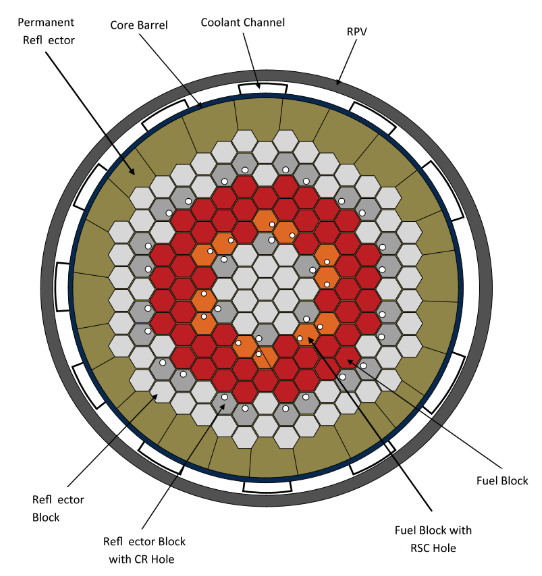
\includegraphics[width=\linewidth]{figures/radial-layout.png}
	% 		\caption{XY-plane.}
	% 	\end{subfigure}
	% 	\begin{subfigure}[t]{0.4\textwidth}
	% 		\centering
	% 		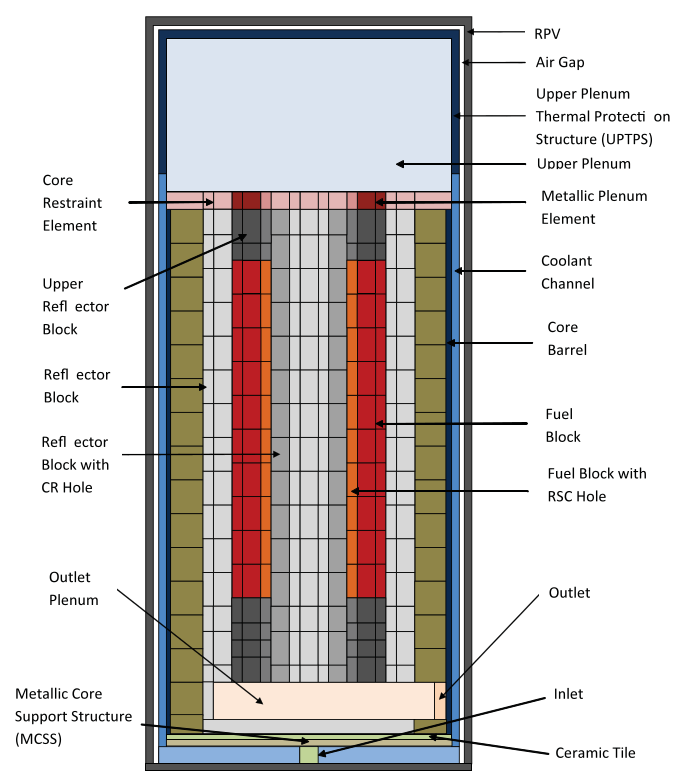
\includegraphics[width=\linewidth]{figures/axial-layout.png}
	% 		\caption{YZ-plane.}
	% 	\end{subfigure}
	% 	\hfill
	% 	\caption{MHTGR reactor layout.}
	% 	\label{fig:layout}
	% \end{figure}

	% \begin{figure}[htbp!]
	% 	\centering
	% 	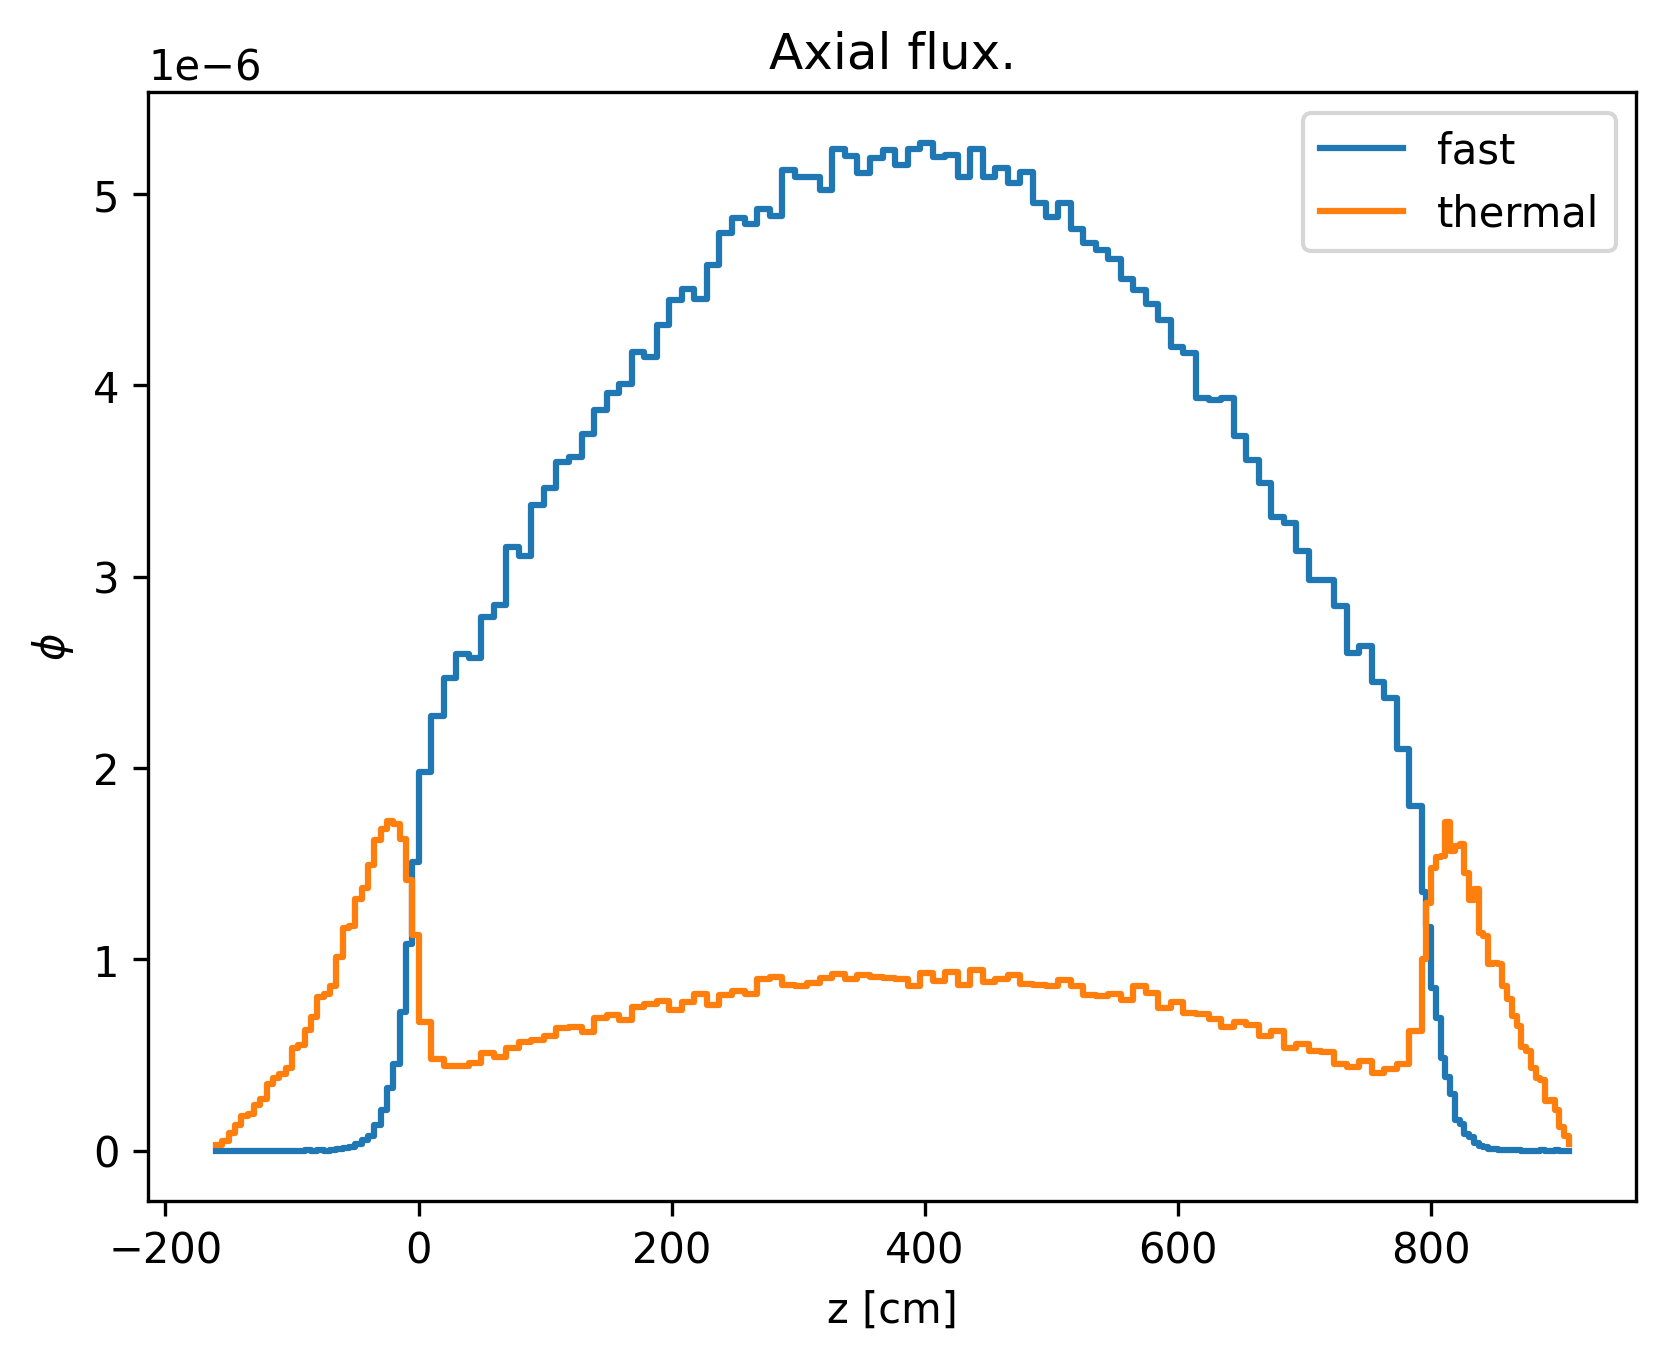
\includegraphics[width=0.6\linewidth]{figures/axial1.png}
	% 	\hfill
	% 	\caption{Neutron flux on the specified fuel channel.}
	% 	\label{fig:axial}
	% \end{figure}

    



\section{Serpent model}
% This will go into tools (tools is actually method)
In 2013, the IAEA launched the Coordinated Research Project (CRP) on Uncertainty Analysis in Modeling (UAM) to study uncertainty propagation in the High Temperature Gas-cooled Reactor (HTGR) analysis chain.

HTGR reactors require core simulation techniques not typically utilized in Light Water Reactor (LWR) analysis due to several unique features, such as double heterogeneous fuel design including tristructural isotropic (TRISO) fuel particles, large graphite quantities, and high operational temperatures.

\cite{bostelmann_criticality_2016}.

A major challenge for neutronics modeling is the double heterogenity present in HTGRs.

The issue of double heterogeneity arises from the introduction of the TRISO fuel particles into the reactor design.
These TRISO particles form the first level of heterogeneity, as they consist of four layers.
The second level of heterogeneity arises from the fuel elements themselves.
The TRISO particles are packed into fuel compacts, which are contained within fuel assemblies that are heterogeneous with the coolant, moderator, and reflector regions.

The computational time required to explicitly model individual TRISO particles in the reactor makes this approach time consuming, costly, and impractical for the majority of applications.
Applying a simple volume homogenization has proven to be insufficient for TRISO particle, due to the resonant self-shielding effect of the kernel and coated layers.

SERPENT is a continuous energy Monte Carlo reactor physics burnup calculation code, developed by VTT Technical Research Centre of Finland and distributed by RSICC in the United States.
SERPENT allows for the explicit modeling of TRISO fuel particles.

\cite{rahnema_whitepaper_2015}.


Talk about the double heterogeneity, that it is important to model it explicitly otherwise a homogenization yields wrong results.
Objective is to address the uncertainties due to double heterogeneity or self-shielding treatment.
cite \ref{strydom_results_2015}
